\documentclass{standalone}
\usepackage{tikz}
\usetikzlibrary{mindmap}


\begin{document}
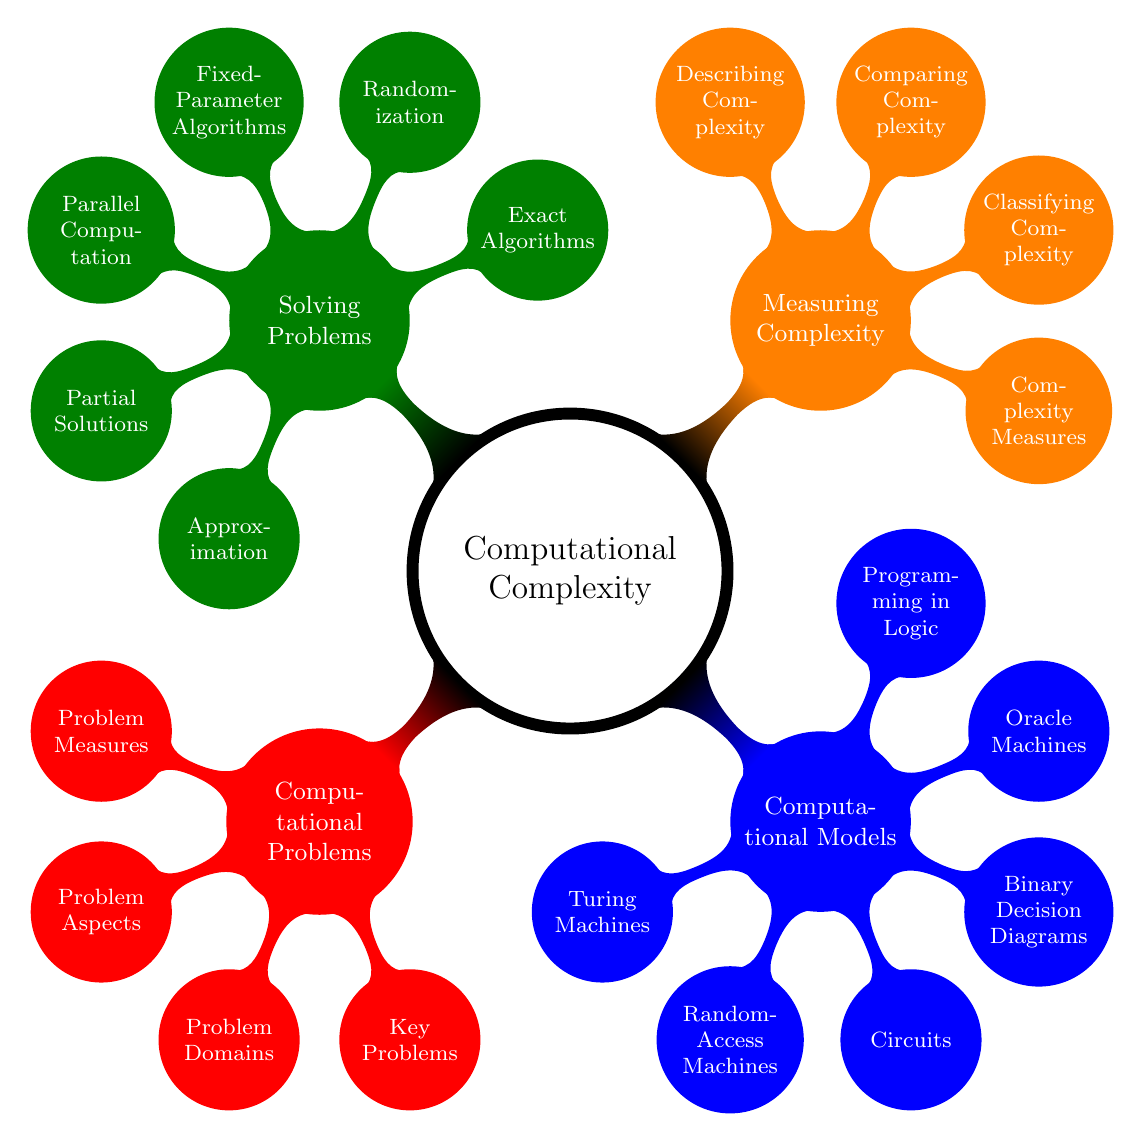
\begin{tikzpicture}[
  mindmap,
  every node/.style={concept, execute at begin node=\hskip0pt},
  root concept/.append style={
    concept color=black, fill=white, line width=1ex, text=black
  },
  text=white, grow cyclic,
  level 1/.append style={level distance=4.5cm,sibling angle=90},
  level 2/.append style={level distance=3cm,sibling angle=45}
]

\node[root concept] {Computational Complexity} % root
child[concept color=red] { node {Computational Problems}
child { node {Problem Measures} }
child { node {Problem Aspects} }
child { node {Problem Domains} }
child { node {Key Problems} }
}
child[concept color=blue] { node {Computational Models}
child { node {Turing Machines} }
child { node {Random-Access Machines} }
child { node {Circuits} }
child { node {Binary Decision Diagrams} }
child { node {Oracle Machines} }
child { node {Programming in Logic} }
}
child[concept color=orange] { node  {Measuring Complexity}
child { node {Complexity Measures} }
child { node {Classifying Complexity} }
child { node {Comparing Complexity} }
child { node {Describing Complexity} }
}
child[concept color=green!50!black] { node {Solving Problems}
child { node {Exact Algorithms} }
child { node {Randomization} }
child { node {Fixed-Parameter Algorithms} }
child { node {Parallel Computation} }
child { node {Partial Solutions} }
child { node {Approximation} }
};
\end{tikzpicture}
\end{document}